\noindent
In the C++ standard template library, there is a class $array< T >$
which offers functions to manipulate arrays. Additionally, in the
EALib a class $array$ is defined. Using this class the dynamical
resizing of arrays is made even more convenient.

\vspace*{5mm}

\noindent
Before explaining how the class $array$ works, I will introduce the
concept of arrays. In the EALib, the array has two vectors. One is the
dimensional vector, in which dimensional data of the array is stored. The
second vector contains the actual content of the array. In this
manual, I will note both vectors by $d$ and $e$, respectively. A rough
explanation is given in Figure \ref{array}.

\begin{center}
\begin{figure}[h]
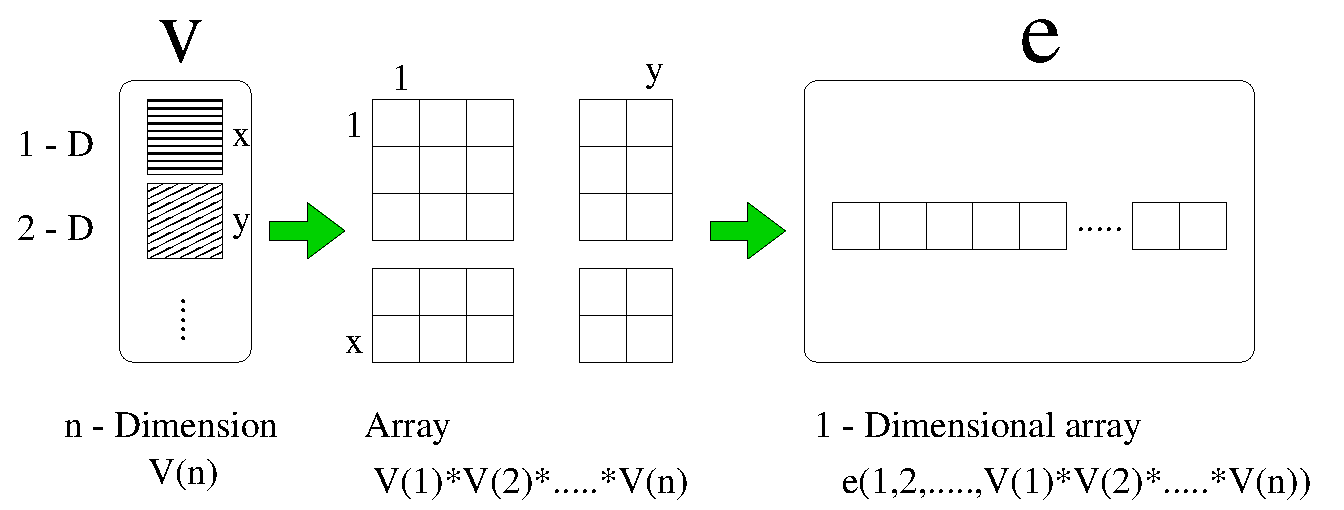
\includegraphics[width=13cm]{array-image.eps}\\
\caption{The organization of arrays in the EALib.}
\label{array}
\end{figure}
\end{center}

\noindent
The vector $d$ contains data about the structure of the array. If $d =
\{ n_1 \}$, this means that the array $e$ is a one dimensional array -
a vector - and the number of elements is $n_1$. If $d = \{ n_1, n_2
\}$, this means that the array $e$ is a two dimensional array - a
matrix - and the number of elements is $n_1 \times n_2$.

\clearpage

\noindent
The vector $e$ contains the actual elements of the array. To explain
this vector, I will use the two dimensional case. The number of
elements are $n_1 \times n_2$. The vector elements from 1 to $n_1$
contain the elements of the first row in the array and the ones from
$n_1+1$ to $2n_1$ contain the elements of the second row, etc.

\vspace*{5mm}

\noindent
In both classes $arraybase$ and $array< Class T>$, the array is
specified by the two vectors $d$ and $e$.

\vspace*{5mm}

\noindent
Caution

\noindent
In C++ programs, the index is from  $0$ to $n-1$ for
$vector[n]$. However, the explanation uses $1$ to $n$. Please bear
this difference in mind !


